\documentclass[oneside,a4paper,12pt]{article}
\usepackage[english,brazilian]{babel}
\usepackage[alf]{abntex2cite}
\usepackage[utf8]{inputenc}
\usepackage[T1]{fontenc}
\usepackage[top=25mm, bottom=20mm, left=20mm, right=20mm]{geometry}
\usepackage{framed}
\usepackage{booktabs}
\usepackage{color}
\usepackage{hyperref}
\usepackage{graphicx}
\usepackage{amsfonts}
\usepackage{subfigure}
\usepackage{enumerate}
\usepackage{float}
\graphicspath{{./Figuras/}}    
\definecolor{shadecolor}{rgb}{0.8,0.8,0.8}
\pagenumbering{arabic}

\usepackage{pgf,tikz}
\usetikzlibrary{arrows}

\usepackage{multicol}
\setlength{\columnseprule}{0pt}

%Cabeçario
\usepackage{fancyhdr}
\lhead{\rightmark}
\renewcommand{\footrulewidth}{0.5pt}

\setlength{\parindent}{1.25cm}%paragrafo

\pagestyle{fancy}
\def\MakeUppercase{} %Fonte minúscula no cabeçario

\pagenumbering{arabic}

\usepackage{amsthm}
\newtheorem{exem}{Exemplo}[section]

\usepackage[skip=10pt]{caption}
\captionsetup{font={stretch=0.4,small}} 

\newcommand{\m}[1]{\({#1}\)}
\newcommand{\M}[1]{\[{#1}\]}
\newcommand{\sol}{\noindent \textbf{Solução }}

\title{\textbf{Equações da Reta}}

\begin{document}
\maketitle

\section{Coeficiente Angular}

Seja uma reta \m{r} no plano cartesiano, e \m{A = (x_a, y_a)} e \m{B = (x_b, y_b)}, dois pontos de \m{r}. O coeficiente angular da reta \m{r}, a tangente do ângulo \m{\alpha}, indicado nas figuras a seguir:

\begin{figure}[!htb]
\center
\begin{multicols}{2}
\includegraphics[width=7cm]{reta1}
\caption{}
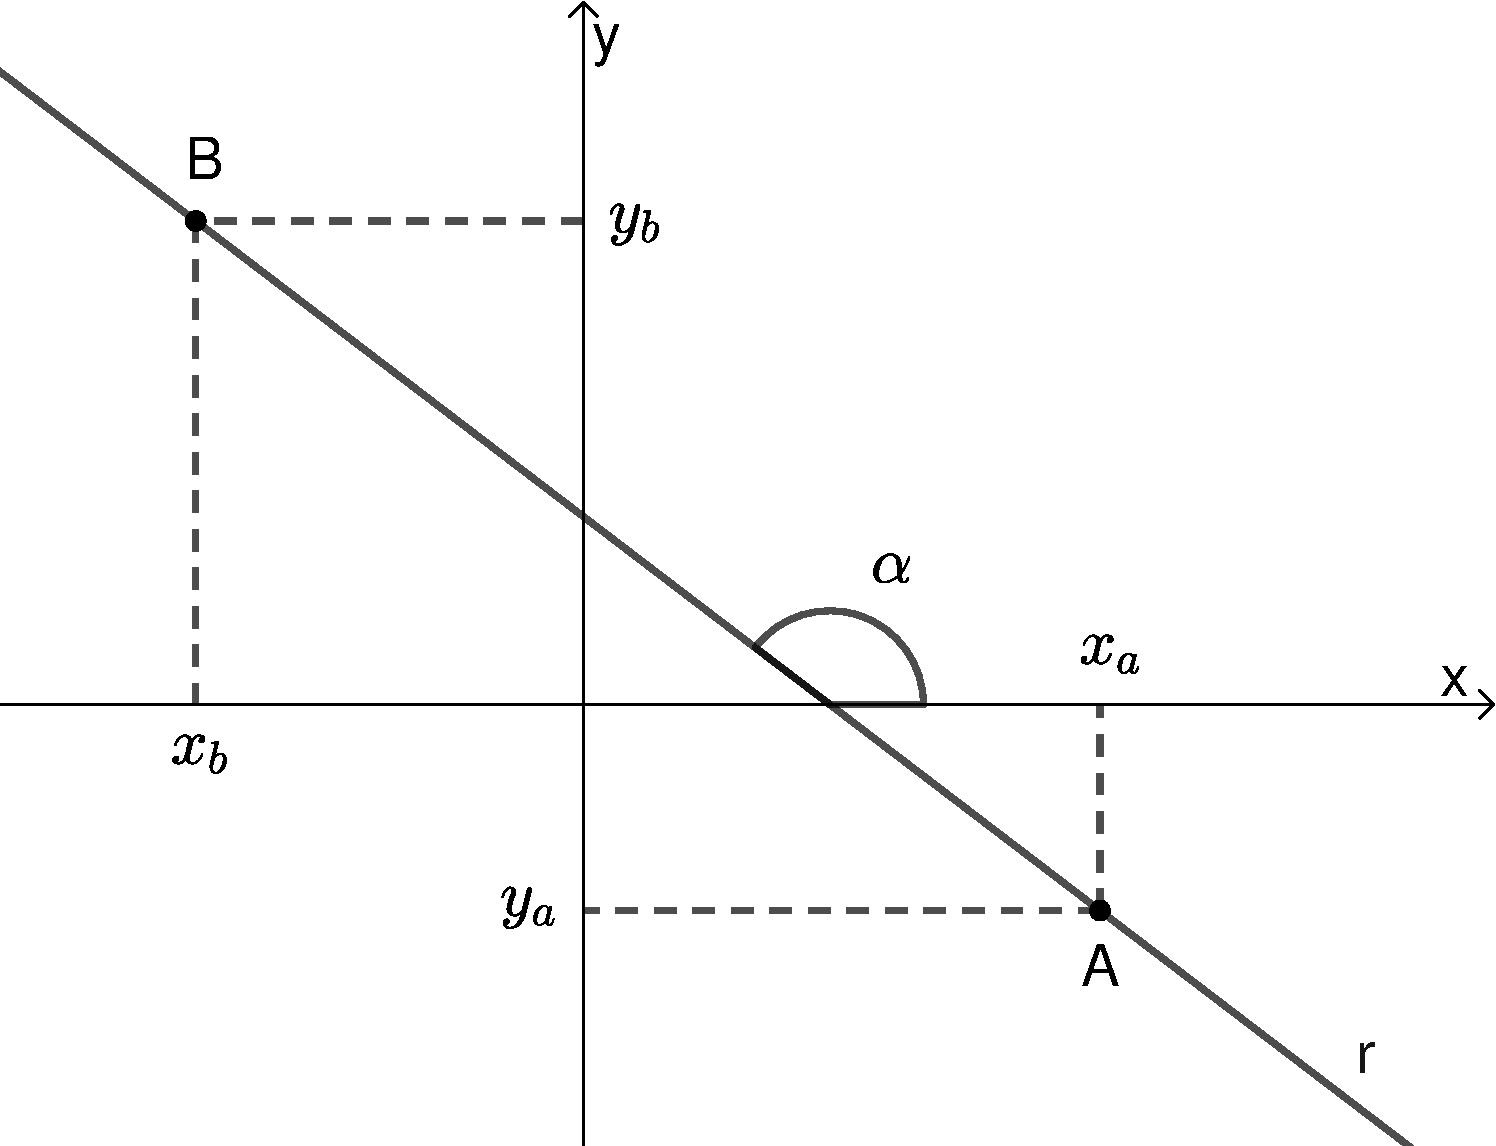
\includegraphics[width=7cm]{reta2}
\caption{}
\end{multicols}
\end{figure}

\noindent O coeficiente angular da reta pode ser calculado usando a seguinte fórmula:

\M{a =  \frac{y_b - y_a}{x_b -  x_a}}

\begin{exemplo}
Calcule o coeficiente angular da reta \m{r} nos planos a seguir:
\end{exemplo}

\end{document}